\chapter[Procesos de Renovación y CTRW]{Procesos de Renovación y Continuous Time Random Walks}


\begin{definicion}
    Definimos un \tbf{paseo aleatorio discreto (P.A.)} (random walk) mediante una sucesión $\{X_i\}_{i=1}^{\infty}$ de variables aleatorias independientes e idénticamente distribuidas (i.i.d.). Estas variables cuantifican la magnitud y dirección de cada salto espacial individual:
    \begin{itemize}
        \item \textbf{Soporte algebraico:} las variables $X_i$ toman valores en $\mathbb{R}$, es decir, no están restringidas a valores no negativos, permitiendo desplazamientos bidireccionales en el espacio.
        \item \textbf{Naturaleza analítica:} las variables $X_i$ pueden ser continuas, caracterizadas mediante funciones de densidad de probabilidad absolutamente continuas con respecto a la medida de Lebesgue sobre la recta real.
    \end{itemize}
\end{definicion}

\observacion{
    Se dice random walk discreto, ya que el proceso se define a través de una \underline{sucesión} \underline{discreta de saltos espaciales}, aunque cada salto individual pueda tomar valores continuos. En contraste, un proceso de difusión continuo (como el Movimiento Browniano) se define mediante una trayectoria continua en el tiempo y el espacio. \\
}

\noindent 
A partir de dicha sucesión, la posición acumulada del proceso tras efectuar exactamente $m$ saltos espaciales viene gobernada por la variable aleatoria suma $Y_m$
\[
Y_m = \sum_{i=1}^{m} X_i
\]

\subsubsection{Modelado bajo Distribuciones Gaussianas}

\noindent 
Supongamos el caso particular en el que los saltos espaciales individuales siguen una distribución normal o Gaussiana clásica, parametrizada por su media $\mu$ y su desviación estándar $\sigma$:
\[
X_i \sim N(\mu, \sigma)
\]
La función de densidad de probabilidad (f.d.p.) del primer salto elemental $X_1$ adopta la estructura analítica:
\[
f_{X_1}(u) = \frac{1}{\sqrt{2\pi}\sigma} \, e^{-\dfrac{(u-\mu)^2}{2\sigma^2}}
\]
Debido a la propiedad de estabilidad de las variables Gaussianas independientes, la función de densidad de la posición acumulada $Y_m$ tras $m$ saltos se determina rigurosamente mediante el operador de convolución de orden $m$, denotado por $f_{X_1}^{*m}(u)$:
\[
f_{Y_m}(u) = f_{X_1}^{*m}(u) = \frac{1}{\sqrt{2\pi m}\sigma} \, e^{-\dfrac{(u-m\mu)^2}{2m\sigma^2}}
\]
Calcularemos ahora la \tbf{esperanza matemática} y la \tbf{varianza} de la variable aleatoria suma $Y_m$ haciendo uso de la linealidad del operador de esperanza matemática y de la propiedad de aditividad de la varianza para variables aleatorias independientes, los dos primeros momentos teóricos de la suma se expanden linealmente con el número de saltos $m$:
\[
\mathbb{E}[Y_m] = \mathbb{E}\left[\sum_{i=1}^{m} X_i\right] = m \, \mathbb{E}[X_1] = m\mu
\]
\[
\text{Var}[Y_m] = \text{Var}\left[\sum_{i=1}^{m} X_i\right] = m \, \text{Var}[X_1] = m\sigma^2
\]

\begin{observacion}
    La identidad fundamental $f_{Y_m}(u) = f_{X_1}^{*m}(u)$ constituye la \textbf{fórmula general para la función de densidad de probabilidad de un solo punto} (one-point probability density function) del proceso suma $Y_m$. Esta relación de convolución iterada es un principio universal para la suma de variables independientes, independientemente de si la ley base es Gaussiana o no. \\
\end{observacion}

\noindent 
Para transformar el paseo aleatorio clásico en un \underline{proceso indexado en tiempo continuo} (CTRW), es imperativo introducir una dimensión temporal estocástica que desacople el número de saltos del tiempo cronológico. \\

\noindent 
\begin{definicion}
    Sea $\{J_i\}_{i=1}^{\infty}$ una sucesión de variables aleatorias estrictamente positivas ($J_i > 0$) e idénticamente distribuidas (i.i.d.), caracterizadas por una función de densidad común $f_{J_1}(u)$. Estas variables modelan los \textbf{tiempos de espera} (waiting times) o retardos que experimenta la partícula inmóvil antes de ejecutar el siguiente salto espacial.
\end{definicion}

\begin{observacion}
    Lo que realmente denota cada variable aleatoria $J_i$ es el tiempo de retención o confinamiento que la partícula permanece en su posición actual antes de efectuar el salto espacial $X_i$. En otras palabras, $J_i$ representa el intervalo de tiempo transcurrido entre el $(i-1)$-ésimo y el $i$-ésimo salto del proceso. \\
\end{observacion}

\begin{definicion}
    El \tbf{instante temporal exacto del $m$-ésimo salto del proceso} viene determinado por la variable aleatoria de tiempo acumulado $T_m$:
    \[
    T_m = \sum_{i=1}^{m} J_i \qquad \text{sujeto a la condición de contorno fija: } T_0 = 0 \quad \text{c.s. (casi seguro)}
    \]
\end{definicion}
\noindent
La variable $T_m$ representa analíticamente un \tbf{proceso de renovación} sobre la línea temporal continua, porque cada vez que la partícula ejecuta un salto, el cronómetro local de espera se destruye y se genera uno nuevo ($J_{i+1}$) con la misma distribución. Es como si el sistema ``olvidara'' el cansancio acumulado y volviera a nacer o a renovarse en cada parada. Los instantes $\{T_1, T_2, T_3, \dots\}$ se denominan científicamente épocas o tiempos de arribo de la renovación. \\

\noindent
Podemos ver una representación gráfica de la evolución temporal del proceso de renovación en el siguiente diagrama, donde se ven reflejadas las naturalezas de ambas variables aleatorias $J_i$ y $T_m$
    \begin{center}
    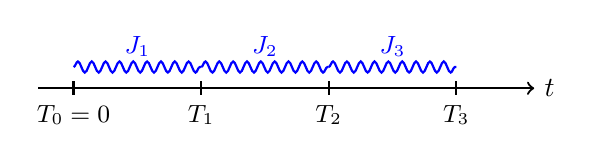
\begin{tikzpicture}[scale=0.9]
        \draw[thick, ->] (-0.5,0) -- (6.5,0) node[right] {$t$};
        \foreach \x in {0,1.8,3.6,5.4} {
            \draw[thick] (\x,0.1) -- (\x,-0.1);
        }
        \node[below, font=\small] at (0,-0.1) {$T_0=0$};
        \node[below, font=\small] at (1.8,-0.1) {$T_1$};
        \node[below, font=\small] at (3.6,-0.1) {$T_2$};
        \node[below, font=\small] at (5.4,-0.1) {$T_3$};
        
        \draw[blue, thick, decorate, decoration={snake, amplitude=2pt, segment length=5pt}] (0,0.3) -- (1.8,0.3) node[midway, above, font=\small] {$J_1$};
        \draw[blue, thick, decorate, decoration={snake, amplitude=2pt, segment length=5pt}] (1.8,0.3) -- (3.6,0.3) node[midway, above, font=\small] {$J_2$};
        \draw[blue, thick, decorate, decoration={snake, amplitude=2pt, segment length=5pt}] (3.6,0.3) -- (5.4,0.3) node[midway, above, font=\small] {$J_3$};
    \end{tikzpicture}
    \end{center}

\begin{ejemplo}  
    Sea $J_1$ una variable aleatoria continua que define el primer tiempo de espera o confinamiento de una partícula en un estado. Supongamos que se rige por una distribución exponencial de parámetro de tasa $\lambda > 0$:
    \[
    J_1 \sim \text{Exp}(\lambda) \implies f_{J_1}(u) = \lambda e^{-\lambda u}, \quad u \ge 0
    \]
    Si consideramos una sucesión $\{J_i\}_{i=1}^{\infty}$ de variables aleatorias independientes e idénticamente distribuidas (i.i.d.) bajo esta misma ley, el instante exacto en el que se ejecuta el $m$-ésimo salto del proceso viene determinado por la variable aleatoria de tiempo acumulado 
    $$T_m = \sum_{i=1}^{m} J_i$$
    Debido a la independencia de los sumandos, la función de densidad de probabilidad (f.d.p.) de $T_m$ se calcula rigurosamente mediante la convolución analítica iterada de orden $m$ de la densidad exponencial base, lo que da origen a la \textbf{Distribución de Erlang}:
    \[
    f_{T_m}(u) = \lambda^m u^{m-1} \frac{e^{-\lambda u}}{(m-1)!}, \quad u \ge 0
    \]
    La distribución de Erlang constituye un caso especial de la distribución Gamma de parámetros continuos cuando el parámetro de forma $m$ se restringe al conjunto de los números enteros positivos ($m \in \mathbb{N}^+$), lo cual permite sustituir la función Gamma abstracta por el operador factorial clásico en el denominador
    \[
    \Gamma(m) = \int_{0}^{\infty} t^{m-1} e^{-t} \, dt = (m-1)!
    \]

    \noindent \textbf{Paralelismo dinámico:} Este esquema temporal es análogo al comportamiento de transición de las Cadenas de Markov (C.M.) convencionales. No obstante, se introduce un cambio de paradigma crítico: los tiempos de retención inter-estado $J_i$ pasan a ser **variables aleatorias continuas**, mientras que en las Cadenas de Markov en tiempo discreto clásicas estaban confinados de forma estricta a distribuciones de soporte **discreto** (distribución geométrica). \\
\end{ejemplo}

 
\begin{definicion}
    Mediante una operación de inversión lógica del paseo aleatorio temporal, definimos el \textbf{proceso de conteo} $N(t)$ indexado en tiempo continuo. Este operador estocástico de valor entero computa el número acumulado (o máximo) de eventos o saltos espaciales completados antes o exactamente en el hito temporal continuo $t \ge 0$:
    \[
    N(t) = \max \{ n \in \mathbb{N}_0 : T_n \le t \}
    \]
\end{definicion}

\begin{definicion}
    Un \textbf{proceso de renovación} es una secuencia de eventos o hitos temporales $\{T_n\}_{n \ge 0}$ donde los tiempos transcurridos entre sucesos consecutivos, definidos como $J_i = T_i - T_{i-1}$ para $i \ge 1$, forman una sucesión de variables aleatorias que cumple rigurosamente las siguientes condiciones:
    \begin{itemize}
        \item Las variables aleatorias $J_1, J_2, J_3, \dots$ son independientes e idénticamente distribuidas (i.i.d.).
        \item El soporte de su función de distribución común $F_J(u)$ está restringido a la semirrecta positiva no nula, es decir:
        \[ P(J_i > 0) = 1 \quad \forall \, i \in \mathbb{N}^+ \]
    \end{itemize}
\end{definicion}

\begin{observacion}
    El proceso de conteo continuo $(N(t))_{t \ge 0}$ que contabiliza cuántos de estos eventos de renovación han acontecido hasta el instante $t$ se denomina, por extensión, el proceso de conteo asociado a dicha renovación.
\end{observacion}

\begin{minipage}{0.45\textwidth}
\begin{center}
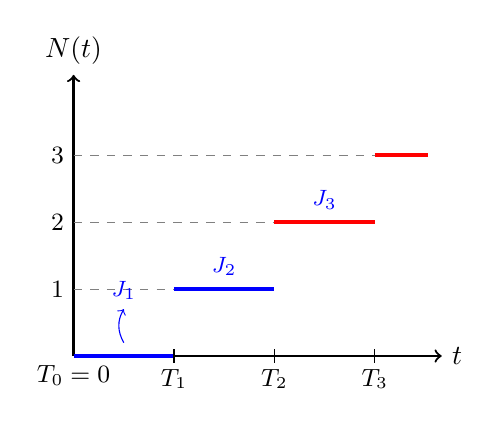
\begin{tikzpicture}[scale=0.85]
    \draw[->, thick] (0,0) -- (5.5,0) node[right] {$t$};
    \draw[->, thick] (0,0) -- (0,4.2) node[above] {$N(t)$};
    
    \draw[dashed, gray] (0,1) -- (1.5,1);
    \draw[dashed, gray] (0,2) -- (3,2);
    \draw[dashed, gray] (0,3) -- (4.5,3);
    
    \draw[ultra thick, blue] (0,0) -- (1.5,0);
    \draw[ultra thick, blue] (1.5,1) -- (3,1);
    \draw[ultra thick, red] (3,2) -- (4.5,2);
    \draw[ultra thick, red] (4.5,3) -- (5.3,3);
    
    \foreach \x in {1.5,3,4.5} \draw (\x,0.1) -- (\x,-0.1);
    \node[below, font=\small] at (0,0) {$T_0=0$};
    \node[below, font=\small] at (1.5,-0.05) {$T_1$};
    \node[below, font=\small] at (3,-0.05) {$T_2$};
    \node[below, font=\small] at (4.5,-0.05) {$T_3$};
    
    \node[left, font=\small] at (0,1) {1};
    \node[left, font=\small] at (0,2) {2};
    \node[left, font=\small] at (0,3) {3};
    
    \draw[blue, ->] (0.75, 0.2) to[bend left] (0.75, 0.7);
    \node[blue, above, font=\footnotesize] at (0.75,0.7) {$J_1$};
    \node[blue, above, font=\footnotesize] at (2.25,1.05) {$J_2$};
    \node[blue, above, font=\footnotesize] at (3.75,2.05) {$J_3$};
\end{tikzpicture}
\end{center}
\end{minipage}
\hfill
\begin{minipage}{0.5\textwidth}
    \noindent \textbf{Propiedades de las Trayectorias muestrales:} \\
    Por naturaleza analítica de los procesos de conteo acumulativos, las trayectorias de $N(t)$ satisfacen la condición matemática de tipo \textbf{c\`{a}dl\`{a}g} (\textit{continue \`{a} droite et limit\'{e} \`{a} gauche}):
    \[
    \text{Las trayectorias son \textbf{continuas por la derecha}}
    \]
    \[
    \text{ y poseen \textbf{límites por la izquierda}.}
    \]
    Físicamente, esto garantiza que en el instante preciso en el que ocurre una renovación u ocurrencia ($t = T_m$), el valor de la variable de conteo absorbe instantáneamente el salto entero superior, reflejando el estado actual del cronómetro.
\end{minipage}

\begin{definicion}[Proceso Compuesto / CTRW]
    El \tbf{paseo aleatorio en tiempo continuo generalizado} se construye formalmente como un proceso compuesto $(Y(t))_{t \ge 0}$, subordinando la cadena de saltos espaciales discretos $Y_m$ al reloj estocástico gobernado por el proceso de conteo de renovaciones $N(t)$:
    \[
    Y(t) = Y_{N(t)} = \sum_{i=1}^{N(t)} X_i
    \]
    donde $X_i$ denota la magnitud aleatoria continua del $i$-ésimo de desplazamiento espacial. \\
\end{definicion}

\begin{observacion}
Las sucesiones discretas independientes de posiciones espaciales acumuladas $(Y_m)_{m \ge 0}$ y de épocas temporales de arribo de renovación $(T_m)_{m \ge 0}$ constituyen de forma aislada, por su diseño recursivo de adición, dos estructuras de Cadenas de Markov discretas en su índice de pasos $m$.
\end{observacion}

\begin{prop}
Si la cadena de posiciones en el espacio $(Y_m)_{m \ge 0}$ y la cadena de tiempos de renovación $(T_m)_{m \ge 0}$ son mutuamente independientes en el sentido estocástico (lo que se denota formalmente mediante la relación de ortogonalidad probabilística $(Y_m)_{m \ge 0} \perp \!\!\! \perp (T_m)_{m \ge 0}$), entonces el vector de estado bidimensional acoplado $(T_m, Y_m)$ hereda y preserva de forma estricta la propiedad de Markov sobre su espacio muestral ordenado.
\end{prop}

\begin{observacion}
A pesar del carácter markoviano del par coordenado indexado por pasos, el proceso final compuesto expandido en el tiempo continuo \textbf{$(Y(t))_{t \ge 0}$ no es un proceso de Markov en general}. Al exhibir tiempos de espera arbitrarios $J_i$, la probabilidad de transición futura depende explícitamente de la memoria del sistema, concretamente del tiempo que lleva la partícula esperando en su posición actual, lo que introduce una dependencia temporal no markoviana. \\
\end{observacion}
\noindent
Esta nota indica que si entramos en el laboratorio y vemos una partícula inmóvil en la casilla $x = 5$. Si queremos calcular la probabilidad de que salte en el próximo segundo, necesitmos hacernos una pregunta crucial: ¿Cuánto tiempo lleva esa partícula durmiendo en esa casilla?
\begin{itemize}
    \item Si la partícula acaba de aterrizar en la casilla hace un microsegundo, su temporizador $J_i$ está entero, por lo que es muy poco probable que salte inmediatamente.
    \item Si la partícula lleva tres horas atrapada en esa misma casilla, su temporizador de espera $J_i$ está a punto de agotarse, por lo que la probabilidad de que salte de forma inminente es altísima.
\end{itemize}
Aquí tenemos la ruptura de Markov, para calcular el futuro, ya no basta con saber el estado presente (la posición $x=5$); necesitas conocer la ``edad'' o el ``tiempo de residencia'' que la partícula acumula en ese lugar. Podemos ver una representación de como avanzaría $Y(t)$ a lo largo del tiempo, con sus periodos de confinamiento y sus saltos espaciales, en el siguiente diagrama:

\begin{center}
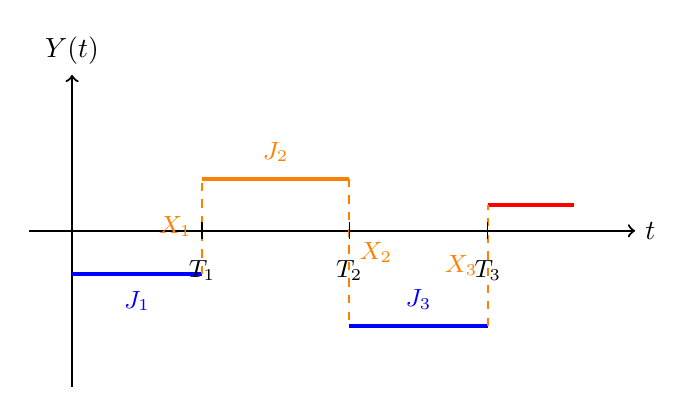
\begin{tikzpicture}[scale=1.1]
    % Ejes del CTRW espacial-temporal
    \draw[->, thick] (-0.5,0) -- (6.5,0) node[right] {$t$};
    \draw[->, thick] (0,-1.8) -- (0,1.8) node[above] {$Y(t)$};
    
    % Trayectorias de confinamiento y saltos espaciales
    \draw[ultra thick, blue] (0,-0.5) -- (1.5,-0.5) node[midway, below=2pt, font=\small] {$J_1$};
    \draw[ultra thick, orange] (1.5,0.6) -- (3.2,0.6) node[midway, above=2pt, font=\small] {$J_2$};
    \draw[ultra thick, blue] (3.2,-1.1) -- (4.8,-1.1) node[midway, above=2pt, font=\small] {$J_3$};
    \draw[ultra thick, red] (4.8,0.3) -- (5.8,0.3);
    
    % Líneas de salto espacial discontinuas (Variables X_i)
    \draw[dashed, orange, thick] (1.5,-0.5) -- (1.5,0.6) node[midway, left, font=\small] {$X_1$};
    \draw[dashed, orange, thick] (3.2,0.6) -- (3.2,-1.1) node[midway, right, font=\small] {$X_2$};
    \draw[dashed, orange, thick] (4.8,-1.1) -- (4.8,0.3) node[midway, left, font=\small] {$X_3$};
    
    % Hitos de Renovación en el Eje de Tiempos
    \draw (1.5,0.1) -- (1.5,-0.1) node[below=4pt, font=\small] {$T_1$};
    \draw (3.2,0.1) -- (3.2,-0.1) node[below=4pt, font=\small] {$T_2$};
    \draw (4.8,0.1) -- (4.8,-0.1) node[below=4pt, font=\small] {$T_3$};
\end{tikzpicture}
\end{center}

\section{Espacio de Probabilidad Filtrado}

\begin{definicion}[Espacio Filtrado]
    La evolución formal de un proceso estocástico en tiempo continuo requiere la introducción de una estructura tetra-dimensional denominada \textbf{espacio de probabilidad filtrado} o espacio adaptado:
    \[
    (\Omega, \mathcal{F}, \{\mathcal{F}_t\}_{t \ge 0}, P)
    \]
    donde la componente $\{\mathcal{F}_t\}_{t \ge 0}$ constituye una \textbf{filtración}, definida analíticamente como una colección o sucesión continua indexada y no decreciente de $\sigma$-álgebras contenidas en el espacio medible global $\mathcal{F}$:
    \[
    \mathcal{F}_s \subseteq \mathcal{F}_t \subseteq \mathcal{F} \quad \forall \, 0 \le s \le t
    \]
    Informalmente, la $\sigma$-álgebra $\mathcal{F}_t$ representa el flujo acumulado de información histórica e instrumental disponible y conocida que ``influye'' y condiciona dinámicamente el comportamiento del proceso hasta el instante cronológico $t$. \\
\end{definicion}

\noindent
Típicamente en la teoría de procesos de saltos, hacemos uso de la \textbf{filtración natural} del sistema, la cual es generada única y exclusivamente por la historia endógena y la trayectoria pasada del propio proceso, es decir, es la que se genera si tu única fuente de información es mirar la trayectoria del propio objeto. No tienes información externa (como el clima o interferencias), solo sabes dónde ha estado la partícula y cuánto ha tardado en moverse.

\vspace{0.4cm}

\begin{minipage}{0.52\textwidth}
\begin{center}
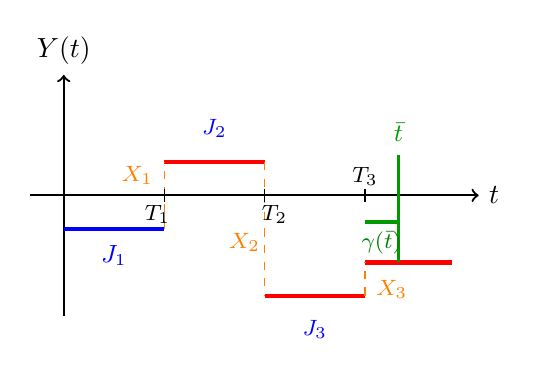
\begin{tikzpicture}[scale=0.85]
    % Ejes del proceso
    \draw[->, thick] (-0.5,0) -- (6.2,0) node[right] {$t$};
    \draw[->, thick] (0,-1.8) -- (0,1.8) node[above] {$Y(t)$};
    
    % Trayectorias horizontales (Estados de retención)
    \draw[ultra thick, blue] (0,-0.5) -- (1.5,-0.5) node[midway, below=2pt] {\small $J_1$};
    \draw[ultra thick, red] (1.5,0.5) -- (3,0.5);
    \draw[ultra thick, red] (3,-1.5) -- (4.5,-1.5);
    \draw[ultra thick, red] (4.5,-1) -- (5.8,-1);
    
    % Líneas discontinuas de los saltos
    \draw[dashed, orange] (1.5,-0.5) -- (1.5,0.5);
    \draw[dashed, orange] (3,0.5) -- (3,-1.5);
    \draw[dashed, orange] (4.5,-1.5) -- (4.5,-1);

    
    % Marcas temporales de renovación
    \node[below, font=\footnotesize] at (1.4,0) {$T_1$};
    \node[below, font=\footnotesize] at (3.15,0) {$T_2$};
    \node[above, font=\footnotesize] at (4.5,0) {$T_3$};
    \node[blue, font=\footnotesize] at (2.25,1) {$J_2$};
    \node[blue, font=\footnotesize] at (3.75,-2) {$J_3$};

    
    \draw (1.5,0.1) -- (1.5,-0.1);
    \draw (3,0.1) -- (3,-0.1);
    \draw (4.5,0.1) -- (4.5,-0.1);
    
    \node[orange, font=\footnotesize] at (1.1,0.3) {$X_1$};
    \node[orange, font=\footnotesize] at (2.7,-0.7) {$X_2$};
    \node[orange, font=\footnotesize] at (4.9,-1.4) {$X_3$};

    
    % Fijación de la ventana de observación \bar{t}
    \draw[thick, green!60!black] (5,0.6) -- (5,-1) node[above=1.4cm, font=\small] {$\bar{t}$};
    \draw[ultra thick, green!60!black] (4.5,-0.4) -- (5,-0.4);
    \node[green!50!black, font=\footnotesize, below] at (4.75,-0.4) {$\gamma(\bar{t})$};
\end{tikzpicture}
\end{center}
\end{minipage}
\hfill
\begin{minipage}{0.45\textwidth}
    Evaluemos el proceso compuesto en una ventana temporal fija e intermedia denotada por $\bar{t}$. De acuerdo con el grafo adjunto, en dicho instante se verifican los siguientes observables algebraicos:
    \begin{align*}
        Y(\bar{t}) &= \sum_{i=1}^{3} X_i \\[0.1cm]
        \mathcal{F}_{\bar{t}} &= \sigma\left(J_1, J_2, J_3, X_1, X_2, X_3, \gamma(\bar{t})\right) \\[0.1cm]
        \gamma(\bar{t}) &= \bar{t} - T_3
    \end{align*}
    La información acumulada en la $\sigma$-álgebra contiene de forma estricta las longitudes de los saltos, los intervalos previos y la fracción de tiempo consumida en el estado actual.
\end{minipage}

\subsection{Definición Clásica de la Propiedad de Markov ($s > t$)}
\noindent
Un proceso estocástico ideal $(X_t)_{t \ge 0}$ satisface la propiedad de falta de memoria si la distribución predictiva condicional del futuro dada la filtración histórica colapsa en la información del presente, es decir
\[
P(X_s \in B \mid \mathcal{F}_t) = P(X_s \in B \mid X_t = x)
\]
lo que viene a ser 
\begin{itemize}
    \item El miembro izquierdo ($P(X_s \in B \mid \mathcal{F}_t)$): calcula la probabilidad de que el proceso en el futuro ($s$) aterrice en un estado $B$, condicionada a toda la bolsa de información histórica acumulada hasta el presente ($\mathcal{F}_t$) (es decir, sabiendo dónde estuvo la partícula en el segundo 1, en el segundo 2, a qué hora dio cada salto, etc.).

    \item El miembro derecho ($P(X_s \in B \mid X_t = x)$): calcula esa misma probabilidad futura, pero condicionada únicamente a saber el valor exacto en el instante presente ($X_t = x$), ignorando por completo el pasado. \\
\end{itemize} 

\noindent
A continuación comentaremos como podemos trabajar con el modelo dado, razonando el porque en parte puede actuar como un proceso markoviano. Para ello usaremos el siguiente diagrama de base

\begin{center}
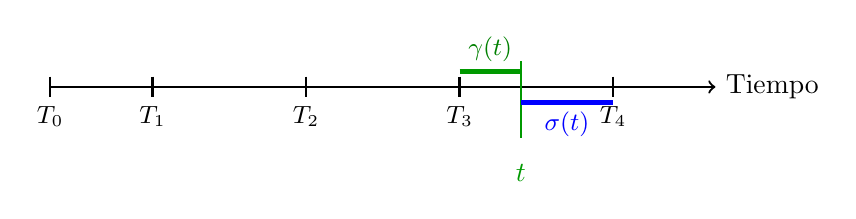
\begin{tikzpicture}[scale=1.3]
    % Línea temporal base
    \draw[->, thick] (0,0) -- (6.5,0) node[right] {Tiempo};
    \foreach \x in {0,1,2.5,4,5.5} {
        \draw[thick] (\x,0.1) -- (\x,-0.1);
    }
    \node[below, font=\small] at (0,-0.1) {$T_0$};
    \node[below, font=\small] at (1,-0.1) {$T_1$};
    \node[below, font=\small] at (2.5,-0.1) {$T_2$};
    \node[below, font=\small] at (4,-0.1) {$T_3$};
    \node[below, font=\small] at (5.5,-0.1) {$T_4$};
    
    % Indicación del hito temporal t de la filtración
    \draw[thick, green!60!black] (4.6,0.25) -- (4.6,-0.5) node[below=0.2cm, font=\bfseries] {$t$};
    
    % Intervalos de Edad y Vida Residual
    \draw[ultra thick, green!60!black] (4,0.15) -- (4.6,0.15);
    \node[green!50!black, font=\small, above] at (4.3,0.15) {$\gamma(t)$};
    
    \draw[ultra thick, blue] (4.6,-0.15) -- (5.5,-0.15);
    \node[blue, font=\small, below] at (5.05,-0.15) {$\sigma(t)$};
\end{tikzpicture}
\end{center}
donde $T_3$ es el último tiempo de arribo de renovación que ocurrió antes o exactamente en el instante $t$, y $T_4$ es el próximo tiempo de arribo que ocurrirá después de $t$. \\

\noindent 
Para analizar el flujo de transición del proceso compuesto $Y(t) \longrightarrow Y(s)$ para un horizonte $s > t$, es imperativo segmentar el intervalo de confinamiento actual mediante dos variables temporales complementarias:
\begin{itemize}
    \item $\gamma(t) = t - T_3$: Es una variable aleatoria determinista respecto a $\mathcal{F}_t$. Representa la \textbf{edad} o el tiempo transcurrido desde el último punto de renovación del sistema hasta el presente $t$. \textbf{Es una variable conocida.}
    \item $\sigma(t) = T_4 - t$: Es una variable aleatoria predictiva fuera del alcance de $\mathcal{F}_t$. Representa el \textbf{tiempo de vida residual} o remanente que la partícula pasará confinada antes de ejecutar el siguiente salto. \textbf{Es una variable desconocida.}
\end{itemize}

\noindent Debido a que el tiempo de vida residual $\sigma(t)$ se encuentra condicionado intrínsecamente por la edad acumulada $\gamma(t)$, la probabilidad de transición futura depende de la memoria de residencia, lo que clasifica a este sistema como un \textbf{PROCESO SEMI-MARKOVIANO}.

\begin{prop}[Vectorización de Markov]
A pesar de que el proceso compuesto espacial $Y(t)$ es inherentemente no markoviano por sí solo, la propiedad de falta de memoria se restaura de forma estricta expandiendo el espacio de estados. El par ordenado bidimensional constituido por la posición y la edad:
\[
(Y(t), \gamma(t))
\]
constituye un \textbf{proceso de Markov} puro en tiempo continuo.
\end{prop}

\begin{prop}[Condición de Markovianidad Pura]
El proceso compuesto unidimensional $Y(t)$ preserva la propiedad de Markov clásica si y solo si los tiempos de inter-arribo o espera $J_i$ se distribuyen bajo una ley exponencial de tasa $\lambda$:
\[
Y(t) \text{ es un proceso de Markov} \iff J_i \sim \text{Exp}(\lambda) \quad \forall \, i \in \mathbb{N}^+
\]
\end{prop}


% \noindent \textbf{\underline{\color{green!50!black}\LARGE DEDUCCIÓN DE LA DISTRIBUCIÓN UNIPUNTUAL DE $Y(t)$}}

% \vspace{0.6cm}

% \noindent \textbf{\large 1. Formalización en el Marco del CTRW Desacoplado}

% \vspace{0.3cm}

% \noindent Consideremos un Paseo Aleatorio en Tiempo Continuo (CTRW) bajo la hipótesis de \textbf{desacoplamiento estricto}. Esto implica que las variables aleatorias de los saltos espaciales $X_i$ y los tiempos de espera $J_i$ son mutuamente independientes. Deseamos hallar la función de distribución acumulada (f.d.a.) unipuntual del proceso compuesto $Y(t) = \sum_{i=1}^{N(t)} X_i$.

% \vspace{0.2cm}

% \noindent Aplicando el teorema de la probabilidad total sobre el soporte discreto del proceso de conteo $N(t)$, la distribución se expande como:
% \begin{align*}
%     F_{Y(t)}(u) &= P(Y(t) \le u) = P\left(\sum_{i=1}^{N(t)} X_i \le u\right) = \\
%     &= \sum_{m=0}^{\infty} P\left(\left.\sum_{i=1}^{m} X_i \le u \,\right|\, N(t) = m\right) P(N(t) = m)
% \end{align*}
% Por la condición de independencia del CTRW desacoplado, el condicionamiento respecto a $N(t)$ en el primer factor se anula. Sustituyendo la posición fija por el paseo aleatorio indexado por pasos $Y_m = \sum_{i=1}^{m} X_i$, y denotando su distribución mediante el operador de convolución espacial iterado de orden $m$ ($F_{X_1}^{*m}$), obtenemos:
% \[
% F_{Y(t)}(u) = \sum_{m=0}^{\infty} P(Y_m \le u) P(N(t) = m) = \sum_{m=0}^{\infty} F_{X_1}^{*m}(u) \cdot P(N(t) = m)
% \]
% Diferenciando término a término respecto a la coordenada espacial $u$, deducimos la función de densidad de probabilidad (f.d.p.) del proceso compuesto, denotada formalmente en el espacio-tiempo como $q(t, u)$:
% \[
% f_{Y(t)}(u) = q(t, u) = \frac{d}{du} F_{Y(t)}(u) = \frac{d}{du} \sum_{m=0}^{\infty} F_{X_1}^{*m}(u) \cdot P(N(t) = m) = \sum_{m=0}^{\infty} f_{X_1}^{*m}(u) \cdot P(N(t) = m)
% \]

% \vspace{0.4cm}

% \noindent \textbf{\large 2. Representación en el Espacio de Fourier (Función Característica)}

% \vspace{0.3cm}

% \noindent Para linealizar el operador de convolución espacial $f_{X_1}^{*m}(u)$, aplicamos la Transformada de Fourier respecto a la variable espacial $u$, obteniendo la función característica del proceso, indexada por el número de onda $k$:
% \[
% \hat{f}_{Y(t)}(k) = \int_{-\infty}^{\infty} q(t, u) e^{iku} \, du = \int_{-\infty}^{\infty} \left( \sum_{m=0}^{\infty} f_{X_1}^{*m}(u) \cdot P(N(t) = m) \right) e^{iku} \, du
% \]
% Haciendo uso de la convergencia de la serie para intercambiar el orden del sumatorio y la integración, y aplicando el teorema de convolución de Fourier (que transforma convoluciones en productos potencias de la densidad base $\hat{f}_{X_1}(k)$), se reduce a:
% \[
% \hat{f}_{Y(t)}(k) = \sum_{m=0}^{\infty} P(N(t) = m) \int_{-\infty}^{\infty} f_{X_1}^{*m}(u) e^{iku} \, du = \sum_{m=0}^{\infty} P(N(t) = m) \left[ \hat{f}_{X_1}(k) \right]^m
% \]

% \strut
% \hfill \rule{\textwidth}{0.5pt} \hfill
% \strut

% \noindent \textbf{\large 3. Núcleo Temporal: Modelado del Proceso de Conteo $P(N(t) = m)$}

% \vspace{0.3cm}

% \noindent El suceso físico de haber realizado exactamente $m$ saltos en el intervalo continuo $[0, t]$ requiere la intersección de dos condiciones temporales: que el $m$-ésimo arribo ocurra antes o en $t$, y que el intervalo de espera subsiguiente $J_{m+1}$ supere el remanente temporal. Sabiendo que $T_m \perp\!\!\!\perp J_{m+1}$:
% \[
% \{N(t) = m\} = \{T_m \le t\} \cap \{J_{m+1} > t - T_m\}
% \]
% Escribiendo la probabilidad mediante el valor esperado de funciones indicadoras y expandiendo la integral conjunta bajo la hipótesis de independencia mutua ($f_{T_m, J_{m+1}}(u, v_1) = f_{T_m}(u)f_{J_1}(v_1)$), tenemos:
% \begin{align*}
%     P(N(t) = m) &= \mathbb{E}\left[ \mathbb{I}_{\{T_m \le t\} \cap \{J_{m+1} > t - T_m\}} \right] = \mathbb{E}\left[ \mathbb{I}_{\{T_m \le t\}} \cdot \mathbb{I}_{\{J_{m+1} > t - T_m\}} \right] = \\
%     &= \int_{0}^{t} du \int_{t-u}^{+\infty} dv_1 \, f_{T_m, J_{m+1}}(u, v_1) = \int_{0}^{t} du \int_{t-u}^{\infty} dv_1 \, f_{T_m}(u) f_{J_1}(v_1) = \\
%     &= \int_{0}^{t} du \, f_{T_m}(u) \int_{t-u}^{\infty} dv_1 \, f_{J_1}(v_1)
% \end{align*}
% Introduciendo la función de supervivencia o complemento de la f.d.a. de los tiempos de espera individuales, definida como $\overline{F}_{J_1}(y) = 1 - F_{J_1}(y) = P(J_1 > y)$, la integral interna se simplifica. Sabiendo que la densidad del tiempo acumulado es la convolución de orden $m$ de la densidad del primer salto ($f_{T_m} = f_{T_1}^{*m}$), la probabilidad se denota abreviadamente como $P(m, t)$:
% \[
% P(m, t) = P(N(t) = m) = \int_{0}^{t} du \, f_{T_1}^{*m}(u) \, \overline{F}_{J_1}(t-u)
% \]
% Esta estructura analítica constituye una \textbf{convolución temporal pura} entre la densidad de arribo $f_{T_1}^{*m}$ y la supervivencia $\overline{F}_{J_1}$.

% \strut
% \hfill \rule{\textwidth}{0.5pt} \hfill
% \strut

% \noindent \textbf{\large 4. Espacio Dual Transformado: La Ecuación de Montroll-Weiss}

% \vspace{0.3cm}

% \noindent Para resolver la convolución temporal, proyectamos la probabilidad $P(m, t)$ al espacio de Laplace respecto a la variable temporal $t$, introduciendo el parámetro de frecuencia compleja $s$:
% \[
% \mathcal{L}[P(m, t)](s) = \widetilde{P}(m, s) = \int_{0}^{\infty} P(m, t) e^{-st} \, dt
% \]
% Por el teorema de convolución de Laplace, la integral temporal de $P(m, t)$ se transforma en un producto algebraico directo de sus componentes en el espacio dual:
% \[
% \widetilde{P}(m, s) = \left[ \widetilde{f}_{J_1}(s) \right]^m \cdot \widetilde{\overline{F}}_{J_1}(s)
% \]
% Retomando la f.d.p. espacial del proceso compuesto $q(t, u) = \sum_{m=0}^{\infty} f_{X_1}^{*m}(u) \, P(N(t) = m)$, aplicamos de manera simultánea la Transformada de Fourier en el espacio ($u \to k$) y la Transformada de Laplace en el tiempo ($t \to s$). Denotando esta representación conjunta como $\widetilde{\hat{q}}(s, k)$, expandimos la serie geométrica resultante:
% \[
% \widetilde{\hat{q}}(s, k) = \sum_{m=0}^{\infty} \left[ \hat{f}_{X_1}(k) \right]^m \widetilde{P}(m, s) = \sum_{m=0}^{\infty} \left[ \hat{f}_{X_1}(k) \right]^m \left[ \widetilde{f}_{J_1}(s) \right]^m \cdot \widetilde{\overline{F}}_{J_1}(s)
% \]
% Extrayendo el factor común de supervivencia independiente del índice de la serie $m$, obtenemos:
% \[
% \widetilde{\hat{q}}(s, k) = \widetilde{\overline{F}}_{J_1}(s) \sum_{m=0}^{\infty} \left[ \hat{f}_{X_1}(k) \widetilde{f}_{J_1}(s) \right]^m
% \]
% Dado que las probabilidades y densidades imponen de forma estricta que $|\hat{f}_{X_1}(k) \widetilde{f}_{J_1}(s)| < 1$ para valores no nulos de los parámetros duales, la serie geométrica infinita converge de manera exacta a la expresión compacta fundamental conocida en física matemática como la \textbf{Ecuación de Montroll-Weiss}:
% \[
% \boxed{\widetilde{\hat{q}}(s, k) = \frac{\widetilde{\overline{F}}_{J_1}(s)}{1 - \hat{f}_{X_1}(k) \widetilde{f}_{J_1}(s)}}
% \]

\section{One-point Distribution of $Y(t)$}
\vspace{0.6cm}

\begin{definicion}[Distribución Unipuntual]
La función $q(t, u)$ representa la \textbf{función de densidad de probabilidad (f.d.p.) de un solo punto} (\textit{one-point PDF}) del proceso compuesto $Y(t)$. Físicamente, determina la probabilidad de encontrar la partícula en la posición espacial exacta $u \in \mathbb{R}$ en un instante de tiempo fijo $t \ge 0$.
\end{definicion}

\noindent 
En el espacio real $(t, u)$, el cálculo de $q(t, u)$ es algebraicamente impracticable debido a que el acoplamiento del CTRW genera infinitas integrales de convolución iteradas. Para resolver el sistema de forma inmediata, se proyecta el proceso hacia un \textbf{dominio dual transformado} aplicando simultáneamente:
\begin{itemize}
    \item \textbf{Transformada de Fourier} sobre la variable espacial: $u \longrightarrow k$ (número de onda).
    \item \textbf{Transformada de Laplace} sobre la variable temporal: $t \longrightarrow s$ (frecuencia compleja).
\end{itemize}


\begin{teo}[Flujo Algorítmico del CTRW Desacoplado]
    La transición de la complejidad infinitesimal del mundo real hacia la simplificación algebraica del espacio dual se sintetiza a través del siguiente mapa de ruta:
    \begin{center}
    \renewcommand{\arraystretch}{1.5}
    \begin{tabular}{lcl}
    \textbf{Mundo Real} $(t, u)$ & $\xrightarrow{\quad\mathcal{F}[\cdot]\text{ e }\mathcal{L}[\cdot]\quad}$ & \textbf{Espacio Dual} $(s, k)$ \\
    \hline
    Densidad de Saltos $f_{X_1}(u)$ & $\longrightarrow$ & Función Característica $\hat{f}_{X_1}(k) = \int_{-\infty}^{\infty} f_{X_1}(u) e^{iku} \, du$ \\
    Densidad de Esperas $f_{J_1}(t)$ & $\longrightarrow$ & Transformada de Laplace $\widetilde{f}_{J_1}(s) = \int_{0}^{\infty} f_{J_1}(t) e^{-st} \, dt$ \\
    Supervivencia Temporal $\overline{F}_{J_1}(t)$ & $\longrightarrow$ & Transformada de Supervivencia $\widetilde{\overline{F}}_{J_1}(s) = \frac{1 - \widetilde{f}_{J_1}(s)}{s}$ \\
    \hline
    \textbf{Densidad de Ocupación $q(t, u)$} & $\longrightarrow$ & \textbf{Solución Algebraica $\widetilde{\hat{q}}(s, k)$} \\
    \end{tabular}
    \end{center}
\end{teo}

\begin{teo}[Ecuación de Montroll-Weiss]
    Bajo la hipótesis de desacoplamiento estricto (independencia mutua entre longitudes de salto y tiempos de espera), la solución exacta de la f.d.p. unipuntual en el espacio dual transformado de Fourier-Laplace colapsa de forma cerrada en la siguiente expresión fundamental:
    \[
    \widetilde{\hat{q}}(s, k) = \frac{\widetilde{\overline{F}}_{J_1}(s)}{1 - \hat{f}_{X_1}(k) \widetilde{f}_{J_1}(s)}
    \]
\end{teo}

\subsubsection{Protocolo de Uso en Problemas Prácticos}
\begin{enumerate}
    \item[\textbf{Paso 1:}] Obtener las transformadas base de los datos del problema: $\hat{f}_{X_1}(k)$ y $\widetilde{f}_{J_1}(s)$.
    \item[\textbf{Paso 2:}] Sustituir directamente dichos términos en la fracción de Montroll-Weiss.
    \item[\textbf{Paso 3:}] Aplicar la transformada inversa de Laplace ($\mathcal{L}^{-1}$) y la inversa de Fourier ($\mathcal{F}^{-1}$) sobre el resultado para regresar al espacio real y obtener la solución explícita $q(t, u)$.
\end{enumerate}

\section{Caso Particular: Tiempos de Espera Exponenciales}

\noindent
Retomamos la Ecuación de Montroll-Weiss para estudiar qué ocurre cuando los tiempos de espera $J_i$ siguen la ley más simple posible: la exponencial. Este caso es especialmente relevante porque es el \textbf{único} que devuelve al CTRW la propiedad de Markov pura (sin necesidad de aumentar el espacio de estados con la edad $\gamma(t)$).

\begin{ejemplo}[Distribución del número de saltos $N(t)$]
    Sea $J_1 \sim \text{Exp}(\lambda)$. Sus transformadas de Laplace son
    \[
    \widetilde{f}_{J_1}(s) = \frac{\lambda}{\lambda+s}, \qquad \widetilde{\overline{F}}_{J_1}(s) = \frac{1}{\lambda+s}.
    \]
    Como $\widetilde{P}(n,s) = \left[\widetilde{f}_{J_1}(s)\right]^n \widetilde{\overline{F}}_{J_1}(s)$, sustituyendo se obtiene
    \[
    \widetilde{P}(n,s) = \frac{\lambda^n}{(\lambda+s)^{n+1}}.
    \]
    Invirtiendo la transformada de Laplace (reconociendo la forma de la densidad Gamma/Erlang desplazada), se llega a
    \[
    \boxed{P(N(t)=n) = e^{-\lambda t}\frac{(\lambda t)^n}{n!}} \quad \Longrightarrow \quad N(t) \sim \text{Poi}(\lambda t).
    \]
\end{ejemplo}

\begin{observacion}
El hecho de que $N(t)$ sea Poisson no es casual: es la \textbf{única} elección de $f_{J_1}$ compatible con la propiedad de falta de memoria de los tiempos de espera. Esto convierte a $N(t)$ en un \textbf{proceso de Poisson}, que cumple
\[
t_1 < t_2 \;\Longrightarrow\; N(t_2)-N(t_1) \overset{d}{=} N(t_2-t_1), \qquad N(t_2)-N(t_1) \;\perp\!\!\!\perp\; N(t_1),
\]
es decir, tiene \textbf{incrementos independientes y estacionarios}. Esta propiedad es la que define a un \textbf{proceso de Lévy}.
\end{observacion}

\section{Límite Difusivo: de la Ecuación de Renovación a la Ecuación del Calor}

\noindent
Existe una versión de la f.d.p. unipuntual escrita directamente en el espacio real $(t,x)$, conocida como \textbf{ecuación de renovación semi-Markoviana}:
\[
\mu(t,x) = \overline{F}_{J_1}(t)\,\delta(x) + \int_{-\infty}^{+\infty} dx' \int_{0}^{t} dt' \; f_{X_1}(x-x')\, f_{J_1}(t-t')\, \mu(x',t').
\]
El primer término representa la probabilidad de que la partícula aún \textbf{no haya saltado} (sigue en $x=0$); el segundo es la convolución espacio-temporal con todas las trayectorias posibles que ya dieron al menos un salto.

\begin{observacion}
Aplicando Fourier-Laplace a esta ecuación se recupera, de forma equivalente, la propia ecuación de Montroll-Weiss:
\[
\widetilde{\hat{\mu}}(s,k) = \frac{1-\widetilde{f}_{J_1}(s)}{s} \cdot \frac{1}{1-\hat{f}_{X_1}(k)\,\widetilde{f}_{J_1}(s)}.
\]
\end{observacion}

\noindent
\textbf{Idea del límite hidrodinámico/difusivo:} si los saltos espaciales tienen media cero y varianza finita, y los tiempos de espera tienen media finita, entonces para $k,s \to 0$ (es decir, observando el proceso a escalas grandes de espacio y tiempo) las transformadas admiten el desarrollo de Taylor
\[
\hat{f}_{X_1}(k) \approx 1 - k^2 + \text{o.t.s.}, \qquad \widetilde{f}_{J_1}(s) \approx 1 - s + \text{o.t.s.}
\]
Sustituyendo y reescalando $k \to c^{1/2}k$, $s \to cs$ con $c \to \infty$, el denominador $1-\hat{f}_{X_1}\widetilde{f}_{J_1}$ se comporta como $c(k^2+s)$, de modo que
\[
\widetilde{\hat{\mu}}(s,k) \xrightarrow[c\to\infty]{} \widetilde{\hat{u}}(s,k) = \frac{1}{k^2+s}.
\]

\begin{teo}[Ecuación de Difusión como límite del CTRW]
La relación $\widetilde{\hat u}(s,k)=\dfrac{1}{k^2+s}$ es equivalente, deshaciendo las transformadas, a invertir Fourier en $k$ y Laplace en $s$ sobre la ecuación algebraica $k^2\hat u + s\hat u = 1$, lo que corresponde al \textbf{problema de Cauchy para la ecuación de difusión}:
\[
\left(\frac{\partial}{\partial t} - \frac{\partial^2}{\partial x^2}\right) u(t,x) = \delta(x)\,\delta(t), \qquad u(0,x)=\delta(x),
\]
cuya solución es el conocido \textbf{núcleo del calor}:
\[
u(t,x) = \frac{1}{\sqrt{2\pi t}}\, e^{-\frac{x^2}{2t}}.
\]
\end{teo}

\begin{observacion}
Este resultado es la versión "macroscópica" del Teorema Central del Límite aplicado al CTRW: bajo escalas grandes, \textbf{cualquier} CTRW desacoplado con saltos de varianza finita y esperas de media finita converge a un Movimiento Browniano, independientemente de la forma exacta de $f_{X_1}$ y $f_{J_1}$ (sólo dependen de ellas a través de sus dos primeros momentos). \\
\end{observacion}

\noindent
Con esto cerramos el bloque de CTRW/renovación.
